% ЕМТ 2023, VI клас — точен LaTeX препис от официалните файлове в Klasirane.com.
% Условия: https://klasirane.com/api/competitions/EMT/All/2023/6%20%D0%BA%D0%BB/probs
% SHA-256 (условия): d8b18df488d80fd67f8c2cf37a2d3a6bd9a82cc7a483bbee05f6ae4e1987fdc0
% Решения: https://klasirane.com/api/competitions/EMT/All/2023/6%20%D0%BA%D0%BB/sol
% SHA-256 (решения): 2323041074fbea3cedaa7c0596c9d0669882a380ae0b61bb61ced35308aaf7bb
% Точковите оценки, правописът, формулировките и видимите печатни грешки са запазени от източника.
% Двете фигури са изрязани без редакция от растеризация на официалния PDF с решенията.

Задача 6.1. Пресметнете числата $a$ и $b$:
$$
a=2{,}023\cdot456+20{,}23\cdot(-24{,}5)-202{,}3\cdot(-7{,}89),
$$
$$
b=\frac1{7\cdot9}+\frac1{9\cdot11}+\frac1{11\cdot13}+\frac1{13\cdot15}+\frac1{15\cdot17}
$$
и намерете числото $x$, за което е изпълнено равенството
$$
5-\frac{1}{\frac15-\frac{1}{5-\frac5x}}=a\cdot b.
$$

Решение. Намираме
$$
a=2{,}023\cdot456+20{,}23\cdot(-24{,}5)-202{,}3\cdot(-7{,}89)=2023\cdot0{,}456-2023\cdot0{,}245+2023\cdot0{,}789=
$$
$$
=2023\cdot(0{,}456-0{,}245+0{,}789)=2023\cdot1=2023;
$$
$$
b=\frac1{7\cdot9}+\frac1{9\cdot11}+\frac1{11\cdot13}+\frac1{13\cdot15}+\frac1{15\cdot17}=\frac12\left(\frac17-\frac19+\frac19-\frac1{11}+\cdots+\frac1{15}-\frac1{17}\right)=
$$
$$
=\frac12\left(\frac17-\frac1{17}\right)=\frac5{119};\qquad a\cdot b=2023\cdot\frac5{119}=85;
$$
$$
5-\frac{1}{\frac15-\frac{1}{5-\frac5x}}=85\Longleftrightarrow
\frac{1}{\frac15-\frac{1}{5-\frac5x}}=-80\Longleftrightarrow
\frac15-\frac{1}{5-\frac5x}=-\frac1{80}\Longleftrightarrow
$$
$$
\Longleftrightarrow\frac{1}{5-\frac5x}=\frac{17}{80}\Longleftrightarrow
5-\frac5x=\frac{80}{17}\Longleftrightarrow
\frac5x=\frac5{17}\Longleftrightarrow x=17.
$$

Оценяване: по 2 точки за намиране на $a$, $b$ и $x$.

Задача 6.2. Правоъгълникът $ABCD$ има лице 555 cm$^2$ и е сглобен от 15 квадрата, както е показано на чертежа.

а) Намерете обиколката на правоъгълника $ABCD$.

б) Намерете лицето на оцветените триъгълници $MNP$ и $MPQ$.

в) Ако отсечките $MP$ и $NQ$ се пресичат в точка $O$, докажете, че $O$ е среда на отсечката $NQ$.

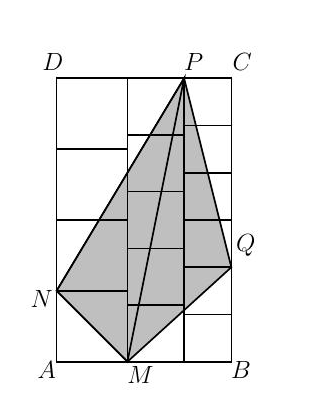
\includegraphics[max width=0.36\textwidth, alt={Правоъгълник ABCD, сглобен от 15 квадрата, с оцветени триъгълници MNP и MPQ}, center]{assets/6-2-squares.png}

Решение. а) (2 точки) Да означим $BC=a$. Тогава страните на квадратите са съответно $\dfrac14a$, $\dfrac15a$ и $\dfrac16a$ и
$$
AB=\left(\frac14+\frac15+\frac16\right)a=\frac{37}{60}a.
$$
Ако $S_{ABCD}=555$ cm$^2$, то
$$
a\cdot\frac{37}{60}a=555\Longleftrightarrow a\cdot a=555:\frac{37}{60}=900,
$$
откъдето $a=30$ cm. Страните на дадения правоъгълник са $BC=30$ cm и $AB=\dfrac{37}{60}\cdot30=18{,}5$ cm, а обиколката му е 97 cm.

б) (2 точки) Изразяваме
$$
S_{AMN}=\frac12\cdot\frac14a\cdot\frac14a=\frac1{32}a^2;\qquad
S_{PDN}=\frac12\cdot\frac34a\cdot\left(\frac14a+\frac15a\right)=\frac{27}{160}a^2;
$$
$$
S_{PCQ}=\frac12\cdot\frac16a\cdot\frac46a=\frac1{18}a^2;\qquad
S_{MBQ}=\frac12\cdot\frac26a\cdot\left(\frac16a+\frac15a\right)=\frac{11}{180}a^2;
$$
$$
S_{AMPD}=\frac12\cdot\left(\frac14a+\frac14a+\frac15a\right)\cdot a=\frac7{20}a^2;\qquad
S_{MBCP}=\frac12\cdot\left(\frac16a+\frac16a+\frac15a\right)\cdot a=\frac4{15}a^2;
$$
$$
S_{MNP}=S_{AMPD}-S_{AMN}-S_{NPD}=\frac7{20}a^2-\left(\frac1{32}+\frac{27}{160}\right)a^2=\frac7{20}a^2-\frac15a^2=\frac3{20}a^2;
$$
$$
S_{MPQ}=S_{MBCP}-S_{CPQ}-S_{MBQ}=\frac4{15}a^2-\left(\frac1{18}+\frac{11}{180}\right)a^2=\frac4{15}a^2-\frac7{60}a^2=\frac3{20}a^2.
$$
Следователно $S_{MNP}=S_{MPQ}=\dfrac3{20}\cdot30^2=135$ cm$^2$.

в) (2 точки) Да означим с $h$ разстоянието от $P$ до $NQ$ и с $t$ – разстоянието от $M$ до $NQ$. Тогава
$$
S_{MNP}=S_{MNO}+S_{PNO}=\frac12\cdot NO\cdot t+\frac12\cdot NO\cdot h=\frac12\cdot NO\cdot(h+t);
$$
$$
S_{MQP}=S_{MQO}+S_{PQO}=\frac12\cdot QO\cdot t+\frac12\cdot QO\cdot h=\frac12\cdot QO\cdot(h+t).
$$
От б) имаме $S_{MNP}=S_{MPQ}$, следователно $\dfrac12\cdot NO\cdot(h+t)=\dfrac12\cdot QO\cdot(h+t)$, от което следва, че $NO=QO$, т.е. $O$ е среда на $NQ$.

Задача 6.3. На един остров живее популация от повече от 100 хамелеони. В понеделник на острова имало само червени и сини хамелеони.

Във вторник 25% от хамелеоните, които в понеделник били сини, станали червени, а 25% от хамелеоните, които в понеделник били червени, станали сини. Така се оказало, че 70% от хамелеоните на острова са сини.

В сряда на острова се родили 10 хамелеони, сини или червени. Така процентът на сините хамелеони на острова станал 68%.

а) Колко процента от хамелеоните на острова са били сини в понеделник?

б) Колко сини хамелеони се родили в сряда и колко хамелеони е имало на острова след това?

в) В четвъртък се срещнали син и червен хамелеон и двата едновременно се оцветили в жълт цвят. По-нататък при всяка среща на два разноцветни хамелеони, те се оцветявали едновременно в третия цвят. Например, ако се срещнели жълт и червен хамелеон, и двата се превръщали в сини. Възможно ли е в края на деня на острова да е имало равен брой червени и жълти хамелеони?

Решение. а) (2 точки) Нека в понеделник имало $x$ сини и $y$ червени хамелеони. Във вторник са $75\%x+25\%y$ сини и $75\%y+25\%x$ червени хамелеони. Така
$$
70\%(x+y)=75\%x+25\%y\Longleftrightarrow x=9y.
$$
Следователно в понеделник имало $x=9y$ сини и $y$ червени хамелеони; общо $10y$, от които сините са били 90%.

б) (3 точки) Тъй като броят на хамелеоните е естествено число, то $25\%y=\dfrac y4$ е естествено, т.е. $y=4a$, където $a$ е естествено число. Изразяваме $x=36a$; общо има $4a+36a=40a$ хамелеони. Във вторник стават $75\%\cdot36a+25\%\cdot4a=28a$ сини и $75\%\cdot4a+25\%\cdot36a=12a$ червени хамелеони.

В сряда на острова се родили 10 хамелеони и те стават общо $40a+10$, от които сините са $68\%=\dfrac{17}{25}$. Ако от новородените хамелиони $b$ са сини, $b\leq10$, имаме
$$
28a+b=\frac{17}{25}\cdot(40a+10)\Longleftrightarrow20a+25b=170\Longleftrightarrow4a+5b=34.
$$
Числото $b$ е четно, не се дели на 4, и не надхвърля 6. Следователно $b=2$, $a=6$ или $b=6$, $a=1$. Във втория случай хамелеоните стават общо 50, а са повече от 100. Следователно $b=2$, $a=6$, което означава, че са се родили 2 сини и 8 червени хамелеони, а общо са станали $40\cdot6+10=250$ хамелеони.

в) (2 точки) Преди срещата на синия и червения хамелеон в четвъртък е имало $\dfrac{17}{25}\cdot250=170$ сини, $250-170=80$ червени и 0 жълти хамелеони.

Нека до края на деня е имало $x$ срещи на жълт и червен, $y$ срещи на жълт и син и $z$ срещи на син и червен хамелеон ($x$, $y$, $z$ са естествени числа или 0). Тогава червените са станали $80-x+2y-z$, а жълтите са станали $2z-x-y$. Равенството
$$
80-x+2y-z=2z-x-y\Longleftrightarrow80=3(z-y)
$$
е невъзможно, тъй като 80 не се дели на 3.

Задача 6.4. Том Сойер трябва да боядиса 10 поредни дъски от една ограда, като изпълни следните изсиквания:

• всяка дъска да е оцветена в бял, син или червен цвят;

• първата и десетата дъски да са бели;

• от две съседни дъски най-много една да е бяла.

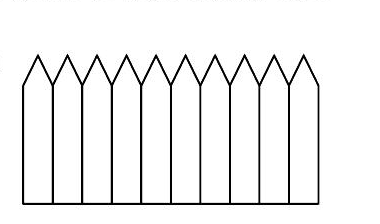
\includegraphics[max width=0.50\textwidth, alt={Десет поредни дъски от ограда}, center]{assets/6-4-fence.png}

а) По колко различни начина Том Сойер може да оцвети оградата?

б) Колко са възможните оцветявания, при които има повече сини, отколкото червени дъски на оградата?

Решение. а) (4 точки) Тъй като от всеки две съседни дъски най-много една е бяла, белите дъски са най-много 5. Тъй като крайните са бели, броят на белите дъски е 2, 3, 4 или 5.

Ако белите дъски са две, първата и десетата, цветът на всяка от останалите 8 дъски може да се избере по 2 начина и получаваме $2^8$ оцветявания.

Нека белите дъски са три. Втората и деветата не са бели, значи вътрешната бяла дъска е с номер 3, 4, 5, 6, 7 или 8, т.е. нейната позиция може да се избере по 6 начина. При всеки такъв избор останалите 7 дъски се оцветяват в син или червен цвят по $2^7$ начина. Получаваме $6\cdot2^7$ оцветявания.

Нека белите дъски са четири. Вътрешните две бели дъски може да са с номера: $(3;a)$, където $a=5;6;7$ или 8; $(4;a)$, където $a=6;7$ или 8; $(5;a)$, където $a=7$ или 8; $(6;8)$. Следователно позицията на двете вътрешни бели дъски може да се избере по $4+3+2+1=10$ начина. При всеки такъв избор останалите 6 дъски се оцветяват в син или червен цвят по $2^6$ начина. Получаваме $10\cdot2^6$ оцветявания.

Нека белите дъски са пет. Вътрешните три бели дъски може да са с номера: $(3;5;7)$, $(3;5;8)$, $(3;6;8)$, $(4;6;8)$. Следователно позицията на трите вътрешни бели дъски може да се избере по 4 начина. При всеки такъв избор останалите 5 дъски се оцветяват в син или червен цвят по $2^5$ начина. Получаваме $4\cdot2^5$ оцветявания.

Общо оцветяванията са
$$
2^8+6\cdot2^7+10\cdot2^6+4\cdot2^5=1792.
$$

б) (3 точки) Първо ще преброим оцветяванията с равен брой червени и сини дъски. Това е възможно само в случаите, когато белите дъски са 2 или 4.

Ако белите дъски са две, първата и десетата, сред останалите 8 дъски мястото на четирите сини може да се избере по $\dfrac{8\cdot7\cdot6\cdot5}{4\cdot3\cdot2\cdot1}=70$ начина.

Ако белите дъски са четири, първата, десетата и две вътрешни, мястото на вътрешните може да се избере по 10 начина (както видяхме в а). При всяки от тези 10 варианта сред останалите 6 дъски мястото на трите сини може да се избере по $\dfrac{6\cdot5\cdot4}{3\cdot2\cdot1}=20$ начина. Така получаваме $10\cdot20=200$ начина.

Следователно при $70+200=270$ оцветявания има равен брой червени и сини дъски.

На всяко оцветяване $C$ с повече сини, отколкото червени дъски, можем да съпоставим оцветяване $C^*$ с повече червени, отколкото сини дъски, като в $C$ преоцветим сините в червени и червените в сини. По този начин оцветяванията с различен брой червени и сини дъски се разделят по двойки; в половината от тези оцветявания, т.е.
$$
\frac{1792-270}{2}=761,
$$
сините дъски са повече от червените.
